\documentclass[Rapport/RPi/RPI.tex]{subfiles}
\begin{document}
\subsubsection{Modultest}
Modultesten for i2c\_interruptDriver er lavet med hjælp fra RPI\_IF klassen fra playerside, der var færdig og testet på dette tidspunkt. Testen brugt til denne klasse blev brugt. Her sendes konstant noget driveren kan læse, og alle mulige beskeder sendt til RPI\_IF udskrives til terminalen. Analog discovery blev brugt til at overvære beskederne sendt over I2C. Her blev logic analyzer brugt i programmet Waveforms. For at teste read blev cat kommandoen brugt i terminalen i lubuntu. Beskeden sendt fra RPI\_IF PSoC'en var 3F i hexadecimal. 3F svarer i ascii er '?'. Dette blev udskrevet til terminalen hvert sekund. 
Til at teste write funktionen blev kommandoen echo i lubuntu brugt. Her blev de forskellige states sendt samt forskellige farvekoder. Dette blev gjort til filen(noden) /dev/playerside2, der har i2c addressen 0x11. Nedenfor i figur \ref{fig:echo_cat} ses et udsnit af terminalen, hvor state IDLE sendes og der læses med cat i 5 sekunder.
\begin{figure}[H]
    \centering 
    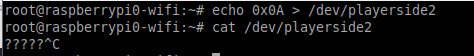
\includegraphics[width=0.5\linewidth]{Rapport/RPi/graphics/i2C_interruptDriver/cat_echo.png}
    \caption{Cat fra noden /dev/playerside2 og echo med state IDLE.}
    \label{fig:echo_cat}
\end{figure}
For at teste om echo beskeden sendt blev der taget et billede af terminalen, som ses i figur \ref{fig:echo_terminal}.
\begin{figure}[H]
    \centering 
    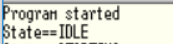
\includegraphics[width=0.4\linewidth]{Rapport/RPi/graphics/i2C_interruptDriver/echo_terminal.PNG}
    \caption{State IDLE sendt til RPI\_IF(PSoC) og udskrevet til terminalen.}
    \label{fig:echo_terminal}
\end{figure}
For at se tests med analog discovery og en mere detaljeret overblik over testen, henvises til bilag.
\end{document}